\documentclass[10pt,aspectratio=43]{beamer}
\usepackage{tikz}
\usetheme{default}
\setbeamertemplate{navigation symbols}{}
\title{Message passing: experiments and bounds}
\subtitle{Generated interaction study}
\author{Research group}
\date{}
\year=2026\month=11\day=5
\newcommand{\fuzzlayerA}[1]{\textrm{#1}}
\newcommand{\fuzzlayerB}[1]{\fuzzlayerA{#1}}
\newcommand{\fuzzterm}[1]{\fuzzlayerB{#1}}
\newcommand{\fuzzpair}[2]{\fuzzterm{#1}: #2}
\newcommand{\fuzzunit}{ms}
\let\fuzzoriginalunit\fuzzunit
\newcommand{\fuzzcoefficient}{2}
\newcommand{\fuzzscale}[2][\fuzzcoefficient]{#1\,#2}
\definecolor{fuzzpaint}{RGB}{255,0,255}
\definecolor{fuzzsecond}{RGB}{18,137,67}
\tikzset{fuzzvertex/.style={draw,rounded corners=1pt,fill=blue!10,inner sep=1pt,minimum width=.35cm,minimum height=.25cm}}
\begin{document}
\section{Message passing}
\begin{frame}[t,shrink=5]{Message passing}{Composed dependencies}
\fuzzpair{Experiment}{Timing: 12\fuzzunit; estimate $\fuzzscale{x}+\fuzzscale[2]{y}$.}\par
{\renewcommand{\fuzzunit}{samples}\let\fuzzterm\textit\fuzzpair{LocalScope}{Timing: 7\fuzzunit.}\par}
\fuzzpair{RestoredScope}{Timing: 11\fuzzunit.}\par
{\scriptsize\color{black}\centering
\begin{enumerate}
\item<1-> \begin{itemize}
\item \textit{The next pass} must preserve the boundary conditions while revisiting dependent values. The next pass must preserve the boundary conditions while revisiting dependent values. The estimate is $\alpha+\beta$.
\item \begin{enumerate}
\item \textrm{A local update} can change the measurements used by several neighboring components.  The estimate is $\alpha+\beta$.
\item \begin{tabular}{lrr}Method&Cost&Error\\\hline
Cached0&5&23\\
Global1&13&29\\
Fresh2&17&15\\
Global3&15&5\\
\end{tabular}
\end{enumerate}
\item \begin{columns}[onlytextwidth,c]
\begin{column}{0.62\textwidth}
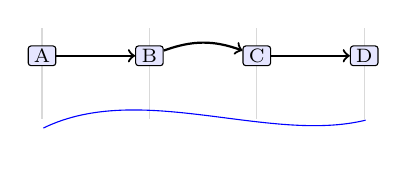
\begin{tikzpicture}[font=\scriptsize]
\begin{scope}[scale=1,rotate=0]

\foreach \x in {0,1,2,3} {\draw[gray!30] (\x*1.364,-.8)--(\x*1.364,.35);}
\node[fuzzvertex] (g8n0) at (0.000,0) {A};
\node[fuzzvertex] (g8n1) at (1.364,0) {B};
\node[fuzzvertex] (g8n2) at (2.728,0) {C};
\node[fuzzvertex] (g8n3) at (4.092,0) {D};
\begin{scope}[xshift=.5pt,yshift=-.5pt]
\draw<1->[->,thick] (g8n0) -- (g8n1);
\draw<1->[->,thick] (g8n1) to[bend left=20] (g8n2);
\draw<1->[->,thick] (g8n2) -- (g8n3);
\draw[blue] (0,-.9) .. controls (1.228,-.3) and (2.864,-1.1) .. (4.092,-.8);
\end{scope}
\end{scope}
\end{tikzpicture}
\end{column}
\begin{column}{0.34\textwidth}
\[\begin{aligned}a+b&=c\\ d-e&=f\end{aligned}\]
\end{column}
\end{columns}
\end{itemize}
\item<2-> \begin{flushright}
\begin{flushright}
\begin{block}{Cache invalidation}
\textrm{The next pass} must preserve the boundary conditions while revisiting dependent values. We compare the proposed solution with a reference computed from the complete input. The estimate is $\sum_{i=1}^{n}x_i$.
\end{block}
\end{flushright}
\end{flushright}
\item<3-> {\footnotesize\color{teal}\raggedright
\only<2->{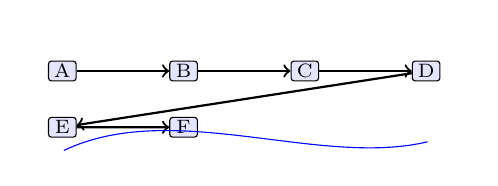
\begin{tikzpicture}[font=\scriptsize]
\begin{scope}[scale=1.1,rotate=0]
\clip (-.4,-1) rectangle (4.700,.5);

\node[fuzzvertex] (g17n0) at (0.000,0) {A};
\node[fuzzvertex] (g17n1) at (1.400,0) {B};
\node[fuzzvertex] (g17n2) at (2.800,0) {C};
\node[fuzzvertex] (g17n3) at (4.200,0) {D};
\node[fuzzvertex] (g17n4) at (0.000,-0.65) {E};
\node[fuzzvertex] (g17n5) at (1.400,-0.65) {F};
\begin{scope}[xshift=.5pt,yshift=-.5pt]
\draw<1->[->,thick] (g17n0) -- (g17n1);
\draw<1->[->,thick] (g17n1) -- (g17n2);
\draw<1->[->,thick] (g17n2) -- (g17n3);
\draw<1->[->,thick] (g17n3) -- (g17n4);
\draw<1->[->,thick] (g17n4) -- (g17n5);
\draw[blue] (0,-.9) .. controls (1.260,-.3) and (2.940,-1.1) .. (4.200,-.8);
\end{scope}
\end{scope}
\end{tikzpicture}}
\par
\begin{tabular}{lrr}Method&Cost&Error\\\hline
Global0&5&11\\
Fresh1&17&26\\
Local2&9&28\\
\end{tabular}\par}
\end{enumerate}\par}
\par 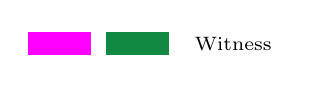
\begin{tikzpicture}[font=\scriptsize]
\fill<2-3>[fuzzpaint] (0,0) rectangle (.8,.3);
\fill<3->[fuzzsecond] (1,0) rectangle (1.8,.3);
\node[anchor=west] at (2,0.15) {Witness};
\end{tikzpicture}
\only<4>{}
\end{frame}
\renewcommand{\fuzzunit}{steps}
\renewcommand{\fuzzcoefficient}{2}
\renewcommand{\fuzzterm}[1]{{\textbf{#1}}}
\section{Iterative refinement}
\begin{frame}[t]{Cache invalidation}
\fuzzpair{MacroStageB}{Timing: 12\fuzzunit, retained: 9\fuzzoriginalunit.}\par
{\renewcommand{\fuzzunit}{local}\fuzzpair{FrameLocal}{Timing: 5\fuzzunit.}\par}
\fuzzpair{FrameRestored}{Timing: 8\fuzzunit; estimate $\fuzzscale{x}$.}\par
\begin{columns}[T]\begin{column}{.46\textwidth}Intermediate results carry both a numerical estimate and an explicit dependency set.\end{column}\begin{column}{.46\textwidth}\begin{itemize}\item Input state\item Updated state\end{itemize}\end{column}\end{columns}
\end{frame}
\renewcommand{\fuzzunit}{s}
\renewcommand{\fuzzcoefficient}{3}
\renewcommand{\fuzzterm}[1]{{\textrm{#1}}}
\section{Cache invalidation}
\begin{frame}[t]{Message passing}
\fuzzpair{MacroStageC}{Timing: 12\fuzzunit, retained: 9\fuzzoriginalunit.}\par
{\renewcommand{\fuzzunit}{local}\fuzzpair{FrameLocal}{Timing: 5\fuzzunit.}\par}
\fuzzpair{FrameRestored}{Timing: 8\fuzzunit; estimate $\fuzzscale{x}$.}\par
\begin{block}{Follow-up}\fuzzterm{A revised value} depends on the preceding frame.\end{block}
\[r_{k+1}=r_k-\alpha d_k\]
\end{frame}
\end{document}
